\documentclass{article}
\usepackage[utf8]{inputenc}
\usepackage[spanish]{babel}
\usepackage{listings}
\usepackage{graphicx}
\graphicspath{ {images/} }
\usepackage{cite}

\begin{document}

\begin{titlepage}
    \begin{center}
        \vspace*{1cm}
            
        \Huge
        \textbf{Taller de memoria}
            
        \vspace{0.5cm}
        \LARGE
            
        \vspace{1.5cm}
            
        \textbf{Daniel Andres Agudelo Garcia}
            
        \vfill
            
        \vspace{0.8cm}
            
        \Large
        Despartamento de Ingeniería Electrónica y Telecomunicaciones\\
        Universidad de Antioquia\\
        Medellín\\
        Septiembre de 2020
            
    \end{center}
\end{titlepage}

\tableofcontents

\vspace{13cm}

\section{Sección introductoria}
Tomando como base del documento Taller - Nociones de la memoria del computador hecho por el profesor Augusto Salazar, tendremos presente que es, para que sirve, como funciona y algunos ejemplos de  cómo es el funcionamiento de las diferentes memorias de computo utilizadas en dispositivos, al igual que su manejo y distribución dentro del mecanismo. \cite{profe}

\vspace{14cm}

\section{Sección de contenido} \label{contenido}
\subsection{¿Que es la memoria del computador?}
Es el dispositivo interno (o en ocasiones se encuentra externo) de un computador el cual se encarga de administrar, retener, memorizar, recapitular información momentánea o permanente, el cual permite mantener disponibles instrucciones o datos para que los microprocesadores puedan leerlas y ejecutarlas.(

\begin{figure}[h]
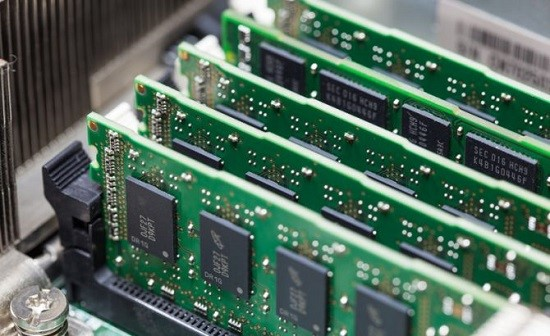
\includegraphics[width=8cm]{que es la memoria.png}
\centering
\caption{Memoria del computador}
\label{fig:que es la memoria}
\end{figure}

\vspace{8cm}

\subsection{Tipos de memoria}
•	MEMORIA CACHE: Esta memoria es donde se guarda y administra de forma temporal datos  del computador que están en continuo uso, alberga poco espacio de información pero es una memoria que libera y gestiona muy rápido dicha información para los microprocesadores. (DOCUMENTO DEL PROFE)

 \vspace{1cm}
 
•	MEMORIA RAM: Esta memoria permite almacenar y leer la información que la CPU necesita mientras está ejecutando un programa, Además, almacena los resultados de las operaciones efectuadas por ella. Este almacenamiento es temporal, ya que la información se borra al apagar el ordenador. \cite{memoria}

 \vspace{1cm}
 
•	MEMORIA ROM: Esta memoria es permanente y es solo de lectura, fue hecha por el fabricante de la maquina (computador) para el funcionamiento técnico del aparato, además es la encargada que apenas se encienda el CPU conecte y verifique que todos los dispositivos estén funcionando correctamente.

 \vspace{1cm}
 
•	DISCO DURO: Son los dispositivos de almacenamiento de datos en los cuales podemos guardar y modificar cualquier tipo de información digital, es la memoria que más espacio tiene disponible pero que a su vez es la más lenta de gestionar por los microprocesadores. \cite{rom}

 \vspace{1cm}

\begin{figure}[h]
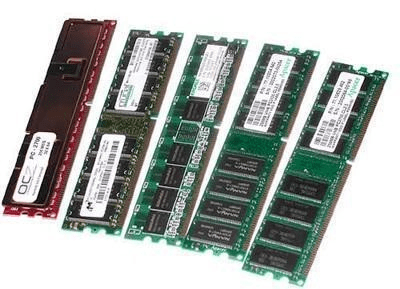
\includegraphics[width=7cm]{tipos.png}
\centering
\caption{Tipos de memoria}
\label{fig:tipos}
\end{figure}

\subsection{Como se gestiona la memoria de un computador}

Es la forma en la que  se trata de “proveer mecanismos para asignar partes de la memoria a los programas que las solicitan, y a la vez, liberar las secciones de memoria que ya no se utilizan para que estén disponibles para otros programas”.  Su labor consiste en llevar un registro de las partes de memoria que se estén utilizando y aquellas que no, con el fin de asignar espacio en memoria a los procesos cuando éstos la necesiten y liberándola cuando terminen. \cite{gestion}

\begin{figure}[h]
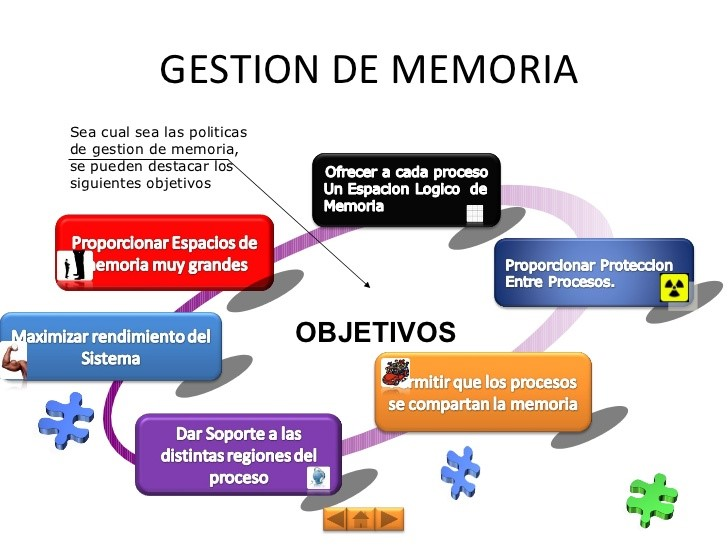
\includegraphics[width=10cm]{gestion.png}
\centering
\caption{Gestion de memoria}
\label{fig:gestion}
\end{figure}

\vspace{5cm}

\subsection{¿Qué hace que una memoria sea más rápida que otra? ¿Por qué esto es importante?}

Hay que partir de la base que mientras más pequeña sea la capacidad de almacenamiento más rápida seria la lectura de los microprocesadores en dicho dispositivo, por ende una memoria cache tiene muy poco almacenamiento pero tiene mucha velocidad de lectura, al contrario de la memoria RAM, que aunque tiene mucho más almacenamiento que una memoria cache, es más lenta su lectura (en el caso de la RAM su velocidad se mide por su frecuencia). 

\vspace{1cm}

Cada memoria tiene su función, como guardar los datos y comando de manera permanentes (memoria ROM) y guardar estos mismos de forma temporal (cache, RAM, etc.) pero lo que hace que un computador sea más veloces es el equilibrio entre la velocidad de los procesadores y la velocidad y espacio de las memorias.  Por ejemplo, cuando compramos una CPU nos fijamos en los GHz que tiene. En el caso de un disco duro, en su velocidad de lectura y escritura, que se mide en MB/s. Y, por supuesto, cuando compramos unas memorias RAM, en su frecuencia, que generalmente se mide en MHz. La teoría nos dice que cuanto más rápida sea esta velocidad más rápido funcionará todo el equipo. Sin embargo, sobre todo en la RAM, existe otro elemento que puede ser más importante que la velocidad: la latencia de la memoria. \cite{importancia}

\vspace{8cm}
\section{Conclusión} \label{conclulsion}
La memoria es el dispositivo más importante para un sistema de computación ya que este se encarga de administrar la información y hacerla ejecutar los programas o archivos que estamos buscando, lo que hace que se vuelva la unidad de almacenamiento junto con los procesadores y microprocesadores, lo que hacen el funcionamiento del dispositivo.

\vspace{1cm}

\bibliographystyle{IEEEtran}
\bibliography{references}

\end{document}
